\documentclass[conference]{IEEEtran}

% Packages that Colton added:
\usepackage{tikz}
\usetikzlibrary{shapes,arrows,shadows,positioning,calc}
\usepackage{listings}
\usepackage{xspace}
\usepackage{balance}

\lstset{
basicstyle=\small\ttfamily,
columns=flexible,
breaklines=true
}
\usepackage{hhline}

% Textual shortcuts
\newcommand{\mr}{{\it mrstudyr}\xspace}
\newcommand{\MR}{\mr}
\newcommand{\mrstudyr}{\mr}
%%%%%%%%%%%%%%%%%%%%%%%%%%%%%%%%%%%%%%%%%%%%%%%%%%%%%%%%%%%%%%%%%%%

% *** GRAPHICS RELATED PACKAGES ***
\ifCLASSINFOpdf
  \usepackage{graphicx}
  % declare the path(s) where your graphic files are
  \graphicspath{{imgs/}}
  % and their extensions so you won't have to specify these with
  % every instance of \includegraphics
  \DeclareGraphicsExtensions{.pdf}
\else
\fi

% *** SUBFIGURE PACKAGES ***
\usepackage{subfig}

\usepackage{stfloats}

% correct bad hyphenation here
\hyphenation{op-tical net-works semi-conduc-tor}

\begin{document}

\title{\mr: Retrospectively Studying the Effectiveness of Mutant Reduction Techniques}

\author{
\IEEEauthorblockN{Colton J. McCurdy}
\IEEEauthorblockA{Allegheny College}
\and
\IEEEauthorblockN{Phil McMinn}
\IEEEauthorblockA{University of Sheffield}
\and
\IEEEauthorblockN{Gregory M. Kapfhammer}
\IEEEauthorblockA{Allegheny College}}

\maketitle

\begin{abstract}
    Mutation testing is a well-known method for measuring a test suite's quality.
    However, due to its computational expense and demand for human interaction,
    mutation testing is often infeasible in practice. To control the demands of
    mutation testing, various reduction strategies have been proposed.
    Although reduction techniques for mutation testing have been described
    in written form, a tool for retrospectively analysing the performance of
    an approach is not available.
    Instead of integrating every reduction approach into an existing mutation testing system and
    individually executing each one, we apply each approach to the data
    collected from a single execution of the entire mutant set.
    We provide a tool, \mr, which enables this retrospective
    comparison of effectiveness for existing mutation testing reduction techniques.
\end{abstract}


\IEEEpeerreviewmaketitle

%!TEX root=../icsme2016-mrstudyr.tex

\section{Introduction}

% Determining the quality of a test suite illustrates how stringently the given program was tested.

% Introduce software testing

Software developers may introduce errors into a program's source code that could result in a human
fatality~\cite{vicente2003programming}. Running a set of tests, frequently called a test suite, often aids in detecting
the faults that cause a program to function incorrectly~\cite{Kapfhammer2010}. Yet, simply testing a program is not
sufficient. In order for testing to establish a confidence in the correctness of the program under test, the test suite
needs to be of a high level of quality~\cite{Kapfhammer2004}.

% Introduce mutation testing and its benefits

Mutation testing is a widely-recognized technique for assessing the quality of a test suite~\cite{gopinath2015mutation}.
While there are many potential faults for a program, mutation testing focuses on those that are ``close'' to the correct
version, with the expectation that they will be representative of all faults~\cite{jia2011analysis}. Of the methods for
evaluating test quality, mutation testing is widely considered the strongest test criterion in terms of its capability
to necessitate the creation of tests that find many faults~\cite{ammann2008introduction}.

% Talk about the limitations of mutation testing

Although mutation testing effectively requires tests to detect faults, it has major drawbacks in its computational cost
and the amount of necessary human interaction, often making it impractical to use~\cite{gopinath2015mutation, Just2011a,
gopinath2015empirical}. A major computational cost of mutation testing comes from executing each test case in a test
suite for the many generated mutants~\cite{Just2012b, offutt1993experimental}. Executing a small, representative set of
mutants against the test suite has previously been proposed as a technique to reduce the cost of mutation
testing~\cite{jia2011analysis, wong1995reducing, offutt1993experimental}; this reduction strategy is categorized by
Offutt and Untch as a ``do fewer'' approach~\cite{offutt2001mutation}.

% Introduce the technique call random mutant sampling

% Due to its simplicity, mutant sampling is considered to be the most cost-effective reduction technique by avoiding
% implementation complexities~\cite{gopinath2015mutation}.  Although it is simple to implement, mutant sampling has still
% been empirically shown to outperform other techniques~\cite{zhang2010operator}.

% TODO: Before the paragraph used operator-based selection in a way that seemed to be incorrect; please check this new
% content. I think that only zhang2013 actually explains this point (and they call it something slightly different).

There are several mutant reduction techniques in the ``do fewer'' category, with mutant sampling being a simple method
that randomly selects a subset of all mutants~\cite{wong1995reducing}. In addition to being conceptually
simple~\cite{gopinath2015mutation}, mutant sampling has been experimentally shown to outperform other more sophisticated
methods~\cite{zhang2010operator}. Two sub-techniques within mutant sampling are called uniform random sampling and
sampling over operators~\cite{gopinath2015mutation, gopinath2015empirical, Zhang2013}. For both of these sub-techniques, a
threshold for the maximum percentage of selected mutants is set to $x$, which is then either applied to the entire set
of mutants or to each set of mutants produced by an operator~\cite{gopinath2015mutation, gopinath2015empirical,
Zhang2013}.

% GMK NOTE: Cut this sentence as it is not precisely the point that we want to main in this paper

% While this way of evaluating reduction techniques is accurate, it is both expensive to implement and perform due to the
% number of times mutation testing needs to be executed.

% GMK NOTE: Here is the source code analysis of the PIT tool using the cloc program (see script in the bin/ directory)

% ./cloc-git https://github.com/hcoles/pitest
% Cloning into 'temp-linecount-repo'...
% remote: Counting objects: 1240, done.
% remote: Compressing objects: 100% (931/931), done.
% remote: Total 1240 (delta 297), reused 557 (delta 122), pack-reused 0
% Receiving objects: 100% (1240/1240), 583.98 KiB | 0 bytes/s, done.
% Resolving deltas: 100% (297/297), done.
% Checking connectivity... done.
% ('temp-linecount-repo' will be deleted automatically)

     % 843 text files.
     % 833 unique files.
     %  63 files ignored.

% http://cloc.sourceforge.net v 1.60  T=1.79 s (456.9 files/s, 36462.9 lines/s)
% -------------------------------------------------------------------------------
% Language                     files          blank        comment           code
% -------------------------------------------------------------------------------
% Java                           780          11126           8087          43030
% Maven                           29            136             23           2287
% XML                              3             33             69            377
% CSS                              1              4              0             36
% Groovy                           2             10              0             32
% YAML                             1              4              1             21
% Bourne Shell                     2              0              0              2
% -------------------------------------------------------------------------------
% SUM:                           818          11313           8180          45785
% -------------------------------------------------------------------------------

% Discuss the challenges associated with these types of analyses, drawing on the code example of PIT

Prior work has found the smallest value of $x$ that still produces a representative set of
mutants~\cite{jia2011analysis, mathur1994empirical}. Yet, these efforts normally required the experimenters to integrate
a reduction technique into an existing mutation testing system before performing a mutation testing
experiment~\cite{demillo1988extended, king1991fortran}. Since mutation testing tools are often complex --- according to
the Count Lines of Code ({\tt cloc}) tool the PIT mutation testing system contains over 43,000 lines of non-commented
Java code and thousands of lines of build and configuration files --- this approach to studying mutant reduction methods
has a high upfront cost. That is, researchers in this field must grasp the complexities of a mutation testing tool
before they can experimentally evaluate new techniques for mutant reduction.

% Retrospectively studying the data collected from a single execution of mutation testing is superior because of its
% minimal upfront costs and the implementation complexities of a target environment are obviated.

% Retrospective analysis is more cost-effective than applying a mutant reduction technique and then evaluating it.  This
% is the case because the expense of mutation testing in retrospective analysis is incurred only once, rather than for
% every reduction technique. Analysing the effectiveness of an approach retrospectively is possible because the necessary
% data can be collected from a prior analysis of all mutants.  This paper introduces \mr, the first and only tool that
% analyses reduction techniques retrospectively.

% GMK NOTE: Even this sentence is not really needed!

% This paper advocates a new way to empirically study mutant reduction methods.

% Introduce the idea of retrospectively studying a mutant reduction method

As a means for obviating the need for researchers to grasp a complex mutation testing system, this paper advances the
idea of retrospectively studying mutant reducers.  After using a tool like PIT to collect data about which operators ran
and what mutants they produced, a retrospective analysis applies strategies like uniform random sampling to the mutant
data, thereby quickly facilitating an understanding of a reduction method's trade-offs. Only after researchers
comprehend how the mutant reducers work in the intended domain must they then grapple with the complexities of the
chosen tool.

% TODO: Is there a place in the paper where we support this claim of the tool being well-documented?

% Okay, now introduce the tool and explain why it is novel

Since retrospective analysis still requires tool support, this paper presents \mr, a tool for evaluating mutant
reduction techniques in retrospect. Accepting data in a generalised format from a single run of a mutation testing
system, \mr~applies mutant reduction strategies and calculates their efficiency and effectiveness. In addition to being
capable of retrospectively analysing mutant reduction techniques from various domains, \mr~is well-documented and has
been released on GitHub under an open-source license.

% GMK NOTE: I have cut all of this content, using some of it in the new streamlined content

% Databases are utilized pervasively for storing everything from batting and pitching statistics of baseball
% players~\cite{lahmanbaseball} to fingerprints and scars of criminals~\cite{ngi}.  Relational databases are an
% efficient and reliable way to store large amounts of data.  The acceptance of relationships between data entries, as
% well as strict structural constraints upheld by the schema are what make relational databases unique.

% The little work testing the integrity constraints of a schema is not because of a sufficient understanding of the topic.
% database schemas~\footnote{http://goo.gl/eZF1mK}.

% Therefore, ensuring that the schemas that are created are also tested is important in upholding the integrity of the
% data contained within the database.

% The database's schema is the artefact responsible for specifying the data to be stored and how it should be structured
% into tables. A series of integrity constraints is what make the database's schema able to ensure values are unique,
% present, subject to domain-specific conditions and maintain referential integrity~\cite{mcminn2016virtual}.  Although
% the schema is the last line of defence for the data contained within a database, little work has sought to test the
% correctness of the integrity constraints~\cite{mcminn2015effectiveness}.

% Using the tool allows you to study mutant reduction in new domains, so go ahead and introduce databases

As studying the mutant data retrospectively removes the need to comprehend the complexities of a target environment,
mutant reduction methods can be extended to new domains such as that of relational database
schemas~\cite{mcminn2016virtual, mcminn2015effectiveness, wright2013efficient}. Ensuring that a database's schema has
correctly specified integrity constraints is important because these entities ensure that only valid data enters the
database. Even though there are \numquestions~questions about databases on StackExchange, the technical question and
answer website~\cite{stackexchange}, little prior work has focused on testing these integrity
constraints~\cite{mcminn2016virtual}.

% A domain that mutation testing has become more prominent in recently is testing database
% schemas~\cite{mcminn2016virtual, mcminn2015effectiveness, wright2013efficient}. However, due to its computation expense,
% it is not widely adopted in industry to test database schemas.  Although mutation testing is used in a variety of
% domains, the reduction techniques can still be utilized, including retrospective analysis~\cite{jia2011analysis,
%   wong1995reducing, offutt1993experimental, offutt2001mutation}.

% GMK NOTE: I have ultimately added in the reference instead of the footnote

% of database schemas~\cite{stackexchange}. Therefore, ensuring that

Since it is important to assess the quality of tests for relational database schemas, recent work has proposed and
evaluated database-aware mutation analysis techniques~\cite{mcminn2016virtual, mcminn2015effectiveness,
wright2013efficient}. Although the presented method and tool are general, this paper illustrates the retrospective study
of mutant reducers and the use of \mr~in the area of mutation analysis for database schemas. In addition to describing
the implementation of \mr~and overviewing results from applying it to the retrospective study of database schema
mutation, this paper inaugurates the public release of this analysis tool. In summary, the key contributions of this
paper are as follows:

\begin{itemize}

  % Although this is a tool paper, perhaps it is acceptable to claim this ideal as a contribution?

  % \item A tool that supports performing mutant reduction methods retrospectively, a way to quickly identify trade-offs
      % without having to understand the complexities of a mutation testing tool.

  % Make a point about the tool and the features that it provides

  % \item A tool that accepts a generalised input format.
  % \item A tool released as a free and open-source R package.

  \item A well-documented and easy-to-use tool, \mr, that:

      \begin{itemize}

          \item supports using mutant reduction methods retrospectively as a way to study trade-offs in efficiency and
            effectiveness without having to understand the implementation of a complex mutation testing tool.

          \item accepts a generalised input format, is extendible to various domains, and is released as a free and
            open-source package in the R programming language.

    \end{itemize}

  % The experimental results (even though preliminary) use real-world database schemas

  \item Using database schemas taken from real-world database-centric applications, preliminary results from using
    \mr, highlighting the benefits of mutant reduction and the ease with which these results may be obtained.

\end{itemize}

%!TEX root=../icsme2016-mrstudyr.tex

% Define the layers to draw the diagram
\pgfdeclarelayer{background}
\pgfdeclarelayer{foreground}
\pgfsetlayers{background,main,foreground}

% Define block styles used later

\tikzstyle{sensor}=[text width=5em,
    text centered, minimum height=2.5em]
\tikzstyle{darksensor}=[draw, fill=black!10, text width=6em,
    text centered, minimum height=2.5em,drop shadow]

% Define distances for bordering
\def\blockdist{1.5}
\def\edgedist{2.5}

\begin{figure}[t]
  \centering
\begin{tikzpicture}[thick,scale=0.85, every node/.style={scale=0.85}]
    \node [] at (0, 5) (map) {\textbf{Mutation Analysis Process}};
    \draw (-4, 4.75) -- (4, 4.75);
    \node [sensor] at (0, 4) (m1) {Generate Mutants};
    \node [sensor] at (0, 2.5) (m2) {Execute Generated Mutants};
    \node [sensor] at (3.25, 3.25) (t1) {Mutation Testing};
    \node [sensor] at (3.25, 1) (t2) {Retrospective Analysis};
    \draw (2, 4.4) -- (2, 1.9);
    \draw (1.7, 4.4) -- (2, 4.4);
    \draw (1.7, 1.9) -- (2, 1.9);
    \node [darksensor] at (0, 1) (m3) {Retrospective Analysis};
    \draw (2, 1.7) -- (2, 0.25);
    \draw (1.7, 1.7) -- (2, 1.7);
    \draw (1.7, 0.25) -- (2, 0.25);

    \path [draw, ->] (m1.south) -- node [above] {}
        (m2.90);
    \path [draw, ->] (m2.south) -- node [above] {}
        (m3.90);
    % \path [draw] (m1.east) -| +(0.3,0) |-node [above] {}
    %     (m2.0);
\end{tikzpicture}
\caption{\label{fig:process}The phases of the mutation analysis process.}
\vspace{-1.5em}
\end{figure}



%!TEX root=../icsme2016-mrstudyr.tex

\section{\textit{mrstudyr}: Mutant Reduction Studier}

%!TEX root=../icsme2016-mrstudyr.tex

\newcommand{\mx}[1]{\mathbf{\bm{#1}}} % Matrix command
\newcommand{\vc}[1]{\mathbf{\bm{#1}}} % Vector command

% Define the layers to draw the diagram
\pgfdeclarelayer{background}
\pgfdeclarelayer{foreground}
\pgfsetlayers{background,main,foreground}

% Define block styles used later

\tikzstyle{sensor}=[draw, fill=black!5, text width=15em,
text centered, minimum height=2.5em,drop shadow]
\tikzstyle{smallsensor}=[draw, fill=black!5, text width=4em,
text centered, minimum height=2.5em,drop shadow]
\tikzstyle{box}=[draw, text width=8em,
text centered, minimum width=17.5em, minimum height=3.5em]
\tikzstyle{calc}=[draw, fill=black!5, text width=2.5em,
text centered, rounded corners, minimum height=2.5em,drop shadow]
\tikzstyle{circle}=[draw, ellipse, fill=black!5, text width=11em,
text centered, minimum height=2.5em, drop shadow]
\tikzstyle{mr}=[draw, fill=black!20, text width=5em,
text centered, minimum height=17em, minimum width = 18em, drop shadow]

% Define distances for bordering
\def\blockdist{1.5}
\def\edgedist{2.5}

\begin{figure}[t]

  \vspace{-.75em}

  \centering
  % SIMPLE
  \begin{tikzpicture}[thick,scale=0.85, every node/.style={scale=0.85}]
    \node [mr] at (0, 0) (mr) {};
    \node [circle] at (0, 3.7) (md) {Original Data};
    \node [sensor] at (0, 2.25) (r) {Reduction Techniques};
    \node [circle] at (0, 0.75) (rmd) {Cumulated Reduced Data};
    \node [sensor] at (0, -0.75) (ra) {Efficiency \& Effectiveness Analysis};
    \node [box] at (0, -2.25) (box) {};
    \node [calc] at (-2.25, -2.25) (ms) {MS};
    \node [calc] at (-0.75, -2.25) (err) {Red.};
    \node [calc] at (0.75, -2.25) (corr) {Corr.};
    \node [calc] at (2.25, -2.25) (err) {Err.};
    \node [sensor] at (0, -3.75) (he) {Human Examination};
    \node [circle] at (0, -5.25) (pr) {Policy Recommendation};

    \path [draw, ->] (md.south) -- node [above] {}
      (r.90);
    \path [draw, ->] (r.south) -- node [above] {}
      (rmd.90);
    \path [draw, ->] (rmd.south) -- node [above] {}
      (ra.90);
    \path [draw, ->] (ra.south) --  node [above] {}
      (box.90);
    \path [draw, ->] (box.south) --  node [above] {}
      (he.90);
    \path [draw, ->] (he.south) -- node [above] {}
      (pr.90);
  \end{tikzpicture}

  \caption{\label{fig:mrstudyr}The inputs and outputs of the \mr~tool.}

  \captionpara{0.5}{0.9}{0.5}{In this figure, the dark square represents the \mr~tool and its constituent parts, a
    rectangle stands for a process, a rectangle with rounded edges is a calculation performed by \mr, and an ellipse
  symbolises a process output.}

  \vspace{-1.8em}
\end{figure}



% Performing mutation testing, displayed in Figure~\ref{fig:process}, is often considered to be too expensive to take

% Review the process of mutation testing, starting with the first part at the top of the diagram

When performed with tools such as Major~\cite{Just2011b}, the process of mutation testing, as displayed in
Figure~\ref{fig:process}, involves the use of operators to generate mutants for a specific program and then the
execution of tests to determine how they kill the mutants. The outcome of this phase is the higher-is-better mutation
score, or the ratio of the number of killed mutants to the number of mutants generated~\cite{Just2011a}. In many cases,
as shown in Figure~\ref{fig:process}, it is necessary to perform various analyses of the mutants. For instance, testers
may want to see which mutants were not killed so as to determine if they are equivalent (i.e., semantically the same as
the original program) or, alternatively, indications of ways to improve the test suite.

% Start to discuss the idea of retrospective mutant analysis for reduction techniques (questions you can answer)

This paper presents another type of mutant analysis: the retrospective study of mutant reduction techniques. Leveraging
data collected during mutation testing (e.g., the name of an operator that produced a mutant, the kill-status of a
mutant, and the costs of producing and analysing a mutant), this method supports the study of mutant reduction
techniques. This type of retrospective analysis allows testers to ask and answer questions like ``what would the
mutation score be if only a random 20\% of the mutants were executed?'' While questions of this nature could be executed
through, for instance, either a manual analysis or a bespoke program, this paper presents \mr, a tool that makes it easy
to effectively pose and answer questions about methods for mutant reduction.

% GMK NOTE: This content has been cut because it was too redundant

% The first of its kind, \mr~is a tool for performing the retrospective analysis of mutant reduction techniques. Upon
% collecting generalised data from performing mutation testing on all mutants, \mr~is capable of determining efficiency
% and effectiveness of well-known mutant reduction techniques specific to the data.

% Talk about the input format of the presented tool, stressing that it is general and useful for many domains

By accepting a generalised input format, the \mr~tool can be utilised in a variety of domains to assess the efficiency
and effectiveness of mutant reduction techniques.  In this paper, we display that \mr~is versatile by conducting a
preliminary study of mutant reduction techniques on mutant data collected from testing database schemas.  However, the
\mr~tool is not limited to analysing mutant data from programs or databases, it can effectively be used in any number
domains. Where mutation testing can be performed, \mr~is capable of analysing reduction techniques.

% Talk about the reduction methods that are implemented in the tool and then explain how easy it is to add new ones
% TODO: Make sure to reference the next section of the paper as it will explain the ways to add methods

The \mr~tool is not limited to the domains where it can be utilised, nor is it restricted
by the reduction approaches it can perform. In the current state, \mr~is able to perform
the most common mutant reduction technique, mutant sampling~\cite{gopinath2015mutation, jia2011analysis, gopinath2015empirical}.
The \mr~tool can be extended to perform specific reduction techniques such as E-Selective
~\cite{offutt1996experimental} --- where only mutants created by the following Mothra operators
are chosen: ABS, UOI, LCR, AOR and ROR~\cite{gopinath2015empirical} or complex reduction techniques
such as mutant clustering, where mutants are chosen based on clustering algorithms~\cite{jia2011analysis}.

% Say that the tool is extensively documented and easy for someone to start using right away

In addition to being extensible in both the domains in which it can be utilized and the
reduction approaches it can perform, \mr~is accompanied with extensive documentation~\cite{tool}.
The documentation includes the necessary commands to get the reader ``up-and-running''
with \mr~quickly and obviates the need to read a poorly-formatted command-line manual page.
The various accepted function calls of the \mr~tool are also provided in the documentation
accompanied by their respective output. Finally, provided in the documentation is a live
asciinema~\cite{asciinema} screencast, displaying usage of the tool.

% GMK NOTE: While this content is interesting and potentially important, I don't think that we have enough space for it!

% The \mr~tool has been released on the popular Git repository hosting service, GitHub~\cite{github}
% under version 3 of the GNU General Public License~\cite{license}. The GNU General Public License
% allows for commercial, patent and private use, as well as distribution of and modification to the tool
% under the condition that anything derived from it is bound by the same conditions as the originally
% released version~\cite{copyleft}.

% vim: ft=tex
%!TEX root=../icsme2016-mrstudyr.tex

\begin{table}[t!]
  \vspace{-0.75em}
  \caption{Sample data analysed in the empirical study.} \label{tbl:study-data}
  \footnotesize
  \centering
  \scalebox{\tablescalefactor}{
    \begin{tabular}{l@{\hskip 4pt}l@{\hskip 4pt}l@{\hskip 4pt}l@{\hskip 4pt}l@{\hskip 4pt}l@{\hskip 6pt}l@{\hskip 0pt}}
      {Identifier} & {DBMS} & {Schema} & {Operator} & {Type} & {Kill} & {Time} \\
      \toprule

      fpbpyn2cnbiinwfyy2mi & SQLite & CoffeeOrders & FKCColumnPairR & NORMAL & true & 59 \\
      fpbpyn2cnbiinwfyy2mi & SQLite & CoffeeOrders & FKCColumnPairR & NORMAL & true & 59 \\
      fpbpyn2cnbiinwfyy2mi & SQLite & CoffeeOrders & FKCColumnPairR & NORMAL & true & 88 \\
      fpbpyn2cnbiinwfyy2mi & SQLite & CoffeeOrders & FKCColumnPairR & NORMAL & true & 54 \\
      fpbpyn2cnbiinwfyy2mi & SQLite & CoffeeOrders & FKCColumnPairE & NORMAL & true & 56 \\
      fpbpyn2cnbiinwfyy2mi & SQLite & CoffeeOrders & FKCColumnPairE & NORMAL & true & 49 \\

      \bottomrule
    \end{tabular}
  }
  \vspace{-1em}
\end{table}

% vim: ft=tex
%!TEX root=../icsme2016-mrstudyr.tex

\begin{table}[t!]
  % \vspace{-0.75em}
    \caption{Schemas analysed in the empirical study.}\label{tbl:study-schemas}
  \vspace{-1em}
  \footnotesize
  \centering
  \scalebox{\tablescalefactor}{
    \begin{tabular}{l@{\hskip -5pt}rrrrrrrr}
      {Schema} & \rot{Tables} & \rot{Columns} & \rot{Checks} & \rot{Foreign Keys} & \rot{Not Nulls} & \rot{Primary Keys} & \rot{Uniques} & \rot{$\sum$Constraints} \\
      \toprule

      CoffeeOrders & 5 & 20 & 0 & 4 & 10 & 5 & 0 & 19 \\
      Employee & 1 & 7 & 3 & 0 & 0 & 1 & 0 & 4 \\
      Inventory & 1 & 4 & 0 & 0 & 0 & 1 & 1 & 2 \\
      Iso3166 & 1 & 3 & 0 & 0 & 2 & 1 & 0 & 3 \\
      JWhoisServer & 6 & 49 & 0 & 0 & 44 & 6 & 0 & 50 \\
      MozillaPermissions & 1 & 8 & 0 & 0 & 0 & 1 & 0 & 1 \\
      NistWeather & 2 & 9 & 5 & 1 & 5 & 2 & 0 & 13 \\
      Person & 1 & 5 & 1 & 0 & 5 & 1 & 0 & 7 \\
      Products & 3 & 9 & 4 & 2 & 5 & 3 & 0 & 14 \\
      \midrule
      Total & 21 & 114 & 13 & 7 & 71 & 21 & 1 & 113 \\

      \bottomrule
    \end{tabular}
  }
  \vspace{-1em}
\end{table}


% \subsection{Retrospective Analysis with \mr}

The next phase in the mutation analysis process is retrospective analysis. In this
phase, mutants are identified as dead or alive. Where a mutant is considered
``dead''---or to have been killed---if when executing the modified version of the source
code the output differed from the original version. Conversely, a mutant remains alive
if the output from the modified version of the source code does not differ from the
original version. More importantly, in this phase of the mutation analysis process,
we are able to evaluate the effectiveness of various reduction techniques.

By retrospectively analysing each reduction technique's effectiveness, we are
able to avoid the cost of performing mutation testing more than once. To alleviate
the additional executions, data from the mutation testing phase needs to be collected.
Displayed in Figure \ref{fig:mrstudyr},
the \mr tool uses the data collected from mutation testing to conduct further analyses
regarding the effectiveness of a reduction technique.

% \subsection{Inputs and Output of \mr}
Displayed in Figure \ref{fig:mrstudyr}, \mr uses the data collected
from mutation testing to conduct further analyses
regarding the efficiency and effectiveness of a reduction technique.

The data provided to the \mr tool must minimally include mutant statuses (e.g., dead or alive),
mutant types (e.g., normal, duplicate, equivalent, or stillborn)
and operators. Moreover, the data can include futher detail about each mutant.
For example, when testing database schemas, the additional data may consist of
the database management system, schema and generation cost of each mutant.

Based on the number of dead and alive mutants after mutation testing,
the \mr tool calculates and associates a mutation score with a set of mutants.
A test suite's mutation score represents its ability to discover faults.
\mr calculates the mutation score for the entire set of mutants to be
used as a baseline for determining each reduced sets' effectiveness.

% \subsection{Calculating Effectiveness with \mr}

\mr performs each reduction technique returning reduced mutant data,
displayed in Figure~\ref{fig:mrstudyr}. The effectiveness of a reduction technique is then evaluated
based on five metrics: mutation score, correlation, the creation-cost reduction percentage
and the mean absolute and root mean squared errors.

These five evaluation metrics help determine how effective a reduced set is at
representing all mutants. \mr calculates mutation score
by dividing the number of killed mutants by the total number of normal---not
equivalent, duplicate or stillborn---mutants. Then, provided by the ``Kendal'' R package,
\mr calculates Kendall's \taub~coefficient---because of its tie-awareness---to
determine the correlation between mutation scores of all mutants and each reduced set~\cite{mcleod2015kendall}.

Kendall's \taub~is a measurement of correlation between -1 and 1, representing
a strong negative or positive correlation, respectively. A measurement
of 0 means that there is no correlation. Additionally, we adopt the
Guildford scale to describe correlation measurements, with the absolute value
of a coefficient being described as ``low'', ``moderate'', ``high'' or ``very high'' when
it is less than 0.4, between 0.4 and 0.7, ranging from 0.7 to 0.9 or 0.9 and above, respectively \cite{inozemtseva2014coverage}.

% Is there a better way to re-word calculating a percentage than provided here?
Next, a percentage representing the reduction magnitude in creation cost for all mutants
and each reduced set is calculated. \mr calculates this by subtracting
the cost of creating the reduced set from the cost of creating all mutants, then
divides that by the cost of creating all mutants. This helps
determine whether performing a reduction technique is cost-effective.

Finally, \mr calculates both mean absolute (MAE) and root mean
squared errors (RMSE). MAE gives an equal weight to all errors allowing for
a high-level understanding, while RMSE emphasises large deviations in mutation scores.
These errors exploit the deviation between the mutation score of all mutants and
the reduced set.


\section{Preliminary Study}

\begin{figure}[!t]

  \centering
  \hspace*{-1em}

  \begin{minipage}{4in}
    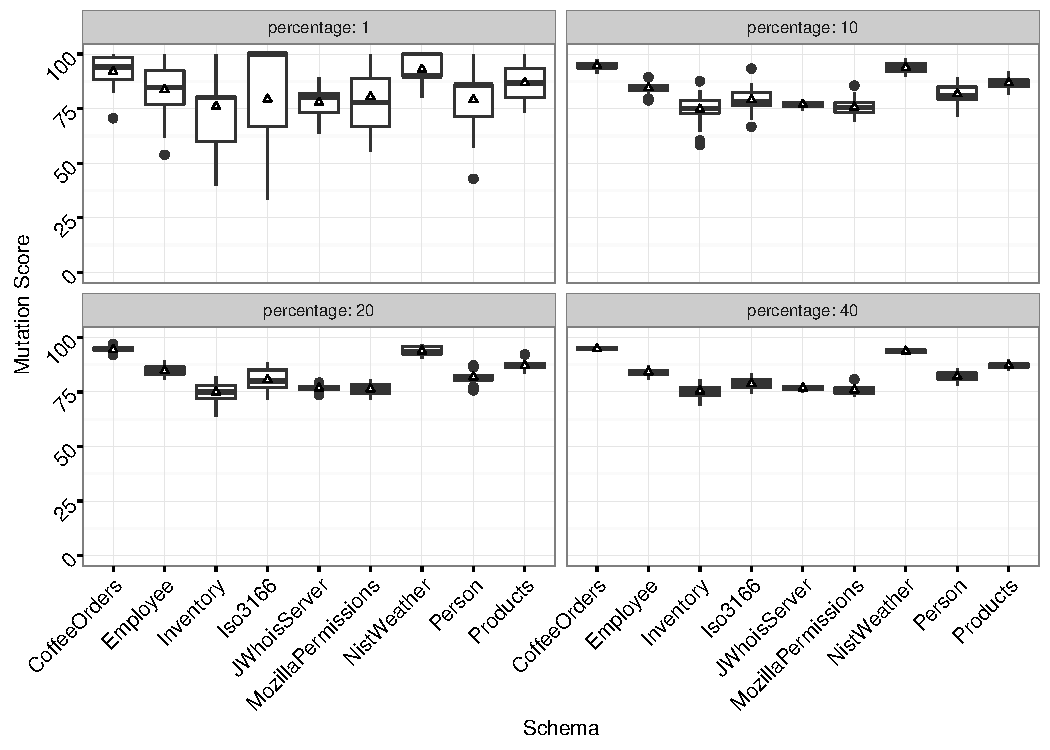
\includegraphics[scale = 0.5]{graphs/schema_vs_ms.pdf}
  \end{minipage}

  \caption{\label{fig:graph}Graph displaying mutation scores for database schemas.}

  \vspace{-1.8em}

\end{figure}


% GMK NOTE: All of this content is really about the design of the experiments and thus it has to be integrated into this
% section (currently, this is still rough content).

We chose these nine schemas because they range in triviality. For example, the MozillaPermissions schema contains a
single constraint, where as the JWhoisServer schema has a total of 50 constraints. This allowed us to evaluate the
policy recommendations made based on the effectiveness of reduction techniques analysed by \mr~for schemas of varying
complexities.

Where Wong and Mathur in their studies~\cite{mathur1994empirical, wong1993mutation} conducted experiments using mutant
sampling with $x$ from $10\%$ to $40\%$ increasing by steps of $5\%$, we chose to analyse $x$ at $1\%$ and then increase
by $10\%$ intervals up to $90\%$. By lowering the granularity of the experiment to $10\%$ intervals instead of $1\%$ or
$5\%$, we reduce the cost of performing retrospective analysis with \mr, while observing similar trends.


\section{Conclusions and Future Work}

% Re-introduce the challenges of mutation testing and summarize what this tool provides

Although mutation testing is well-recognized as a way to assess test suite quality, it may be too costly to practically
use. As such, various methods have been developed to decrease the cost of mutation testing. Performing these reduction
techniques in the past has required researchers and experimenters to incorporate a reduction method into an, often
complex, mutation testing tool. \mr~alleviates the burden of implementing each approach by retrospectively analysing
reduction techniques, a potentially more cost-effective method.

% TODO: It would be ideal if this paragraph could point out the experimental results in this paper

% Summarize some of the key features of the tool and then talk about how it is released and enables future work

By retrospectively analysing the data collected from prior analysis of all mutants, the \mr~tool is able to reduce the
upfront human-implementation costs and obviate the need for researchers and industrialists to understand the domain
complexities associated with understanding a mutation testing system. Furthermore, \mr~provides an
easy-to-use and rapid way to assess the efficiency and effectiveness of mutant reduction methods. In addition to being
detailed in this paper, \mr~has been released under an open-source license on a GitHub site that features extensive
documentation and a screencast~\cite{tool}. In future work, we plan to extend the functionality of \mr~by integrating
additional mutant reduction techniques, thereby allowing for a more comprehensive comparison of the techniques'
efficiency and effectiveness.



\newpage

\balance
\bibliographystyle{IEEEtran}
\bibliography{IEEEabrv,bibliography}
\end{document}
